%%-----------------------------------------------------------------------------
%%
%%                                   Sean Mauch
%%                       California Institute of Technology
%%                          (a) 2000 No Rights Reserved
%%
%%-----------------------------------------------------------------------------

\flushbottom

%% CONTINUE: decide to go with either "region" or "domain"






%%============================================================================
%%============================================================================
\chapter{Contour Integration and the Cauchy-Goursat Theorem}






Between two evils, I always pick the one I never tried before.

\begin{flushright}
  - Mae West
\end{flushright}







%%=============================================================================
\section{Line Integrals}


In this section we will recall the definition of a line integral
in the Cartesian plane.  In the next section we
will use this to define the contour integral in the complex plane.


\paragraph{Limit Sum Definition.}
First we develop a limit sum definition of a line integral.
Consider a curve $C$ in the Cartesian plane joining the points $(a_0,b_0)$
and $(a_1,b_1)$.  We partition the curve into $n$ segments with the points
$(x_0,y_0), \ldots, (x_n,y_n)$  where the first and last points are at
the endpoints of the curve.  We define the differences, $\Delta x_k = x_{k+1} - x_k$ and 
$\Delta y_k = y_{k+1} - y_k$, and let $(\xi_k,\psi_k)$ be points on the 
curve between $(x_k,y_k)$ and $(x_{k+1},y_{k+1})$.  This is shown pictorially in 
Figure~\ref{cart_curve_c}.

\begin{figure}[htb!]
  \begin{center}
    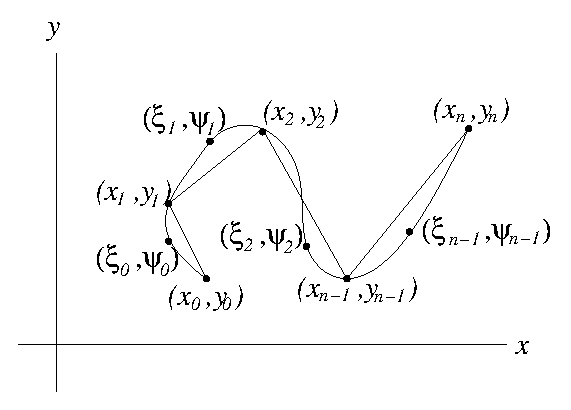
\includegraphics[width=0.5\textwidth]{fcv/integration/cart_curve_c}
  \end{center}
  \caption{A curve in the Cartesian plane.}
  \label{cart_curve_c}
\end{figure}

Consider the sum
\[
\sum_{k = 0}^{n-1} \left( P(\xi_k, \psi_k) \Delta x_k + Q(\xi_k, \psi_k) \Delta y_k \right),
\]
where $P$ and $Q$ are continuous functions on the curve.
($P$ and $Q$ may be complex-valued.)
In the limit as each of the $\Delta x_k$ and $\Delta y_k$ approach zero
the value of the sum, (if the limit exists), is denoted by
\[
\int_C P(x,y) \,\dd x + Q(x,y)\,\dd y.
\]
This is a \textit{line integral} along the curve $C$.
\index{line integral}
The value of the line integral depends on the functions $P(x,y)$ and 
$Q(x,y)$, the endpoints of the curve and the curve $C$.
We can also write a line integral in vector notation.
\[
\int_C \mathbf{f}(\mathbf{x}) \cdot \,\dd \mathbf{x}
\]
Here $\mathbf{x} = (x, y)$ and $\mathbf{f}(\mathbf{x}) = ( P(x,y), Q(x,y) )$.





\paragraph{Evaluating Line Integrals with Parameterization.}
Let the curve $C$ be parametrized by $x = x(t)$, $y = y(t)$ for 
$t_0 \leq t \leq t_1$.  Then the differentials on the curve are
$\dd x = x'(t)\,\dd t$ and $\dd y = y'(t)\,\dd t$.
Using the parameterization we can evaluate a line integral in terms of 
a definite integral.
\[
\int_C P(x,y) \,\dd x + Q(x,y)\,\dd y = 
\int_{t_0}^{t_1} \big( P(x(t), y(t)) x'(t) + Q(x(t), y(t)) y'(t) \big)\,\dd t
\]



\begin{Example}
  Consider the line integral
  \[
  \int_C x^2 \,\dd x + (x+y)\,\dd y,
  \]
  where $C$ is the semi-circle from $(1,0)$ to $(-1,0)$ in the upper 
  half plane.  We parameterize the curve with $x = \cos t$, $y = \sin t$ for 
  $0 \leq t \leq \pi$.
  \begin{align*}
    \int_C x^2 \,\dd x + (x+y)\,\dd y
    &= \int_0^\pi \left( \cos^2 t (-\sin t) + (\cos t + \sin t) \cos t
    \right)\,\dd t 
    \\
    &= \frac{\pi}{2} - \frac{2}{3}
  \end{align*}
\end{Example}
















%%=============================================================================
\section{Contour Integrals}



\paragraph{Limit Sum Definition.}
We develop a limit sum definition for contour integrals.  
It will be analogous to the definition for line integrals 
except that the notation is cleaner in complex variables.
Consider a contour $C$ in the complex plane joining the points $c_0$
and $c_1$.  We partition the contour into $n$ segments with the points
$z_0, \ldots, z_n$ where the first and last points are at
the endpoints of the contour.  We define the differences $\Delta z_k = z_{k+1} - z_k$
and let $\zeta_k$ be points on the 
contour between $z_k$ and $z_{k+1}$.  Consider the sum
\[
\sum_{k = 0}^{n-1} f(\zeta_k) \Delta z_k,
\]
where $f$ is a continuous function on the contour.
In the limit as each of the $\Delta z_k$ approach zero
the value of the sum, (if the limit exists), is denoted by
\[
\int_C f(z) \,\dd z.
\]
This is a \textit{contour integral} along $C$.
\index{contour integral}
\index{line integral!complex}

We can write a contour integral in terms of a line integral.
Let $f(z) = \phi(x,y)$.  ($\phi : \mathbb{R}^2 \mapsto \mathbb{C}$.)
\begin{gather}
  \nonumber
  \int_C f(z) \,\dd z = \int_C \phi(x,y) (\dd x + \imath \,\dd y) 
  \\
  \int_C f(z) \,\dd z = \int_C (\phi(x,y)\,\dd x + \imath \phi(x,y)\,\dd y)  
  \label{eqn comp line int line int}
\end{gather}
Further, we can write a contour integral in terms of two real-valued 
line integrals.  Let $f(z) = u(x,y) + \imath v(x,y)$.
\begin{gather}
  \nonumber
  \int_C f(z) \,\dd z = \int_C (u(x,y) + \imath v(x,y)) (\dd x + \imath \,\dd y) 
  \\
  \int_C f(z) \,\dd z = \int_C (u(x,y)\,\dd x - v(x,y)\,\dd y)  
  + \imath \int_C (v(x,y)\,\dd x + u(x,y)\,\dd y)
  \label{comp_line_int_real_line_int}
\end{gather}




\paragraph{Evaluation.}
Let the contour $C$ be parametrized by $z = z(t)$ for 
$t_0 \leq t \leq t_1$.  Then the differential on the contour is
$\dd z = z'(t)\,\dd t$.
Using the parameterization we can evaluate a contour integral in terms of 
a definite integral.
\[
\int_C f(z) \,\dd z
= \int_{t_0}^{t_1} f(z(t)) z'(t)\,\dd t
\]










\begin{Example}
  \label{three_comp_line_int}
  Let $C$ be the positively oriented unit circle about the origin in the 
  complex plane.  Evaluate:
  \begin{enumerate}
  \item
    $\int_C z\,\dd z$
  \item
    $\int_C \frac{1}{z}\,\dd z$
  \item
    $\int_C \frac{1}{z}\,|\dd z|$
  \end{enumerate}

  In each case we parameterize the contour and then do the integral.
  \begin{enumerate}
    %%
    %%
  \item
    \[
    z = \e^{\imath \theta}, \quad \dd z = \imath \e^{\imath \theta} \,\dd \theta 
    \]
    \begin{align*}
      \int_C z\,\dd z 
      &= \int_0^{2\pi} \e^{\imath \theta} \imath \e^{\imath \theta}\,\dd \theta 
      \\
      &= \left[ \frac{1}{2} \e^{\imath 2 \theta} \right]_0^{2 \pi} 
      \\
      &= \left( \frac{1}{2} \e^{\imath 4 \pi} - \frac{1}{2} \e^{\imath 0} \right) 
      \\
      &= 0
    \end{align*}
    %%
    %%
  \item
    \[
    \int_C \frac{1}{z}\,\dd z 
    = \int_0^{2 \pi} \frac{1}{\e^{\imath \theta}} \imath \e^{\imath \theta}\,\dd \theta
    = \imath \int_0^{2 \pi} \,\dd \theta = \imath 2 \pi
    \]
    %%
    %%
  \item
    \[
    |\dd z|  = \left| \imath \e^{\imath \theta} \,\dd \theta \right| 
    = \left| \imath \e^{\imath \theta} \right|  | \dd \theta |
    = |\dd \theta|
    \]
    Since $\dd \theta$ is positive in this case, $|\dd \theta| = \dd \theta$.
    \[
    \int_C \frac{1}{z}\,|\dd z|
    = \int_0^{2 \pi} \frac{ 1 }{ \e^{\imath \theta} }\,\dd \theta
    = \left[ \imath \e^{-\imath \theta} \right]_0^{2 \pi}
    = 0
    \]
  \end{enumerate}
\end{Example}




%%---------------------------------------------------------------------------
\subsection{Maximum Modulus Integral Bound}


The absolute value of a real integral obeys the inequality
\[
\left| \int_a^b f(x) \,\dd x \right| \leq \int_a^b | f(x) | \,|\dd x|
\leq (b - a) \max_{a \leq x \leq b} |f(x)|.
\]
Now we prove the analogous result for the modulus of a contour integral.
\begin{align*}
  \left| \int_C f(z) \,\dd z \right|
  &= \left| \lim_{\Delta z \to 0} \sum_{k = 0}^{n-1} f(\zeta_k) \Delta z_k \right| 
  \\
  &\leq \lim_{\Delta z \to 0} \sum_{k = 0}^{n-1} \left| f(\zeta_k) \right|  \left| \Delta z_k \right| 
  \\
  &= \int_C |f(z)| \,|\dd z| 
  \\
  &\leq \int_C \left( \max_{z \in C} |f(z)| \right) \,|\dd z| 
  \\
  &= \left( \max_{z \in C} |f(z)| \right) \int_C |\dd z| 
  \\
  &= \left( \max_{z \in C} |f(z)| \right) \times (\mathrm{length of}\ C)
\end{align*}



%% CONTINUE: Should I use max or lub?


\begin{Result}
  \index{integral bound!maximum modulus}
  \index{maximum modulus integral bound}
  \label{max_mod_int_bound}
  \textbf{Maximum Modulus Integral Bound.}
  \[
  \left| \int_C f(z) \,\dd z \right| \leq \int_C |f(z)| \,|\dd z|
  \leq \left(\max_{z \in C} |f(z)| \right) (\mathrm{length of}\ C)
  \]
\end{Result}



%% CONTINUE: properties
%% CONTINUE: examples













%%=============================================================================
\section{The Cauchy-Goursat Theorem}




Let $f(z)$ be analytic in a compact, closed, connected domain $D$.
We consider the integral of $f(z)$ on the boundary of the domain.
\[
\int_{\partial D} f(z) \,\dd z
= \int_{\partial D} \psi(x,y)  (\dd x + \imath\,\dd y)
= \int_{\partial D} \psi \,\dd x + \imath \psi \,\dd y
\]
Recall Green's Theorem.
%% CONTINUE: reference
\[
\int_{\partial D} P \,\dd x + Q \,\dd y
= \int_D (Q_x - P_y)\,\dd x\,\dd y
\]
If we assume that $f'(z)$ is continuous, we can apply Green's Theorem 
to the integral of $f(z)$ on $\partial D$.
\[
\int_{\partial D} f(z) \,\dd z
= \int_{\partial D} \psi \,\dd x + \imath \psi \,\dd y
= \int_D (\imath \psi_x - \psi_y) \,\dd x\,\dd y
\]
Since $f(z)$ is analytic, it satisfies the Cauchy-Riemann equation 
$\psi_x = - \imath \psi_y$.  The integrand in the area integral, $\imath \psi_x - \psi_y$, is zero.  
Thus the contour integral vanishes.
\[
\int_{\partial D} f(z) \,\dd z = 0
\]
This is known as \textit{Cauchy's Theorem}.  The assumption that 
$f'(z)$ is continuous is not necessary, but it makes the proof much simpler
because we can use Green's Theorem.  If we remove this restriction the result
is known as the \textit{Cauchy-Goursat Theorem}.  The proof of this
result is omitted.
%% CONTINUE: add a section for the proof.



%% CONTINUE: compact?
\begin{Result}
  \label{cauchy-goursat theorem}
  \textbf{The Cauchy-Goursat Theorem.}
  If $f(z)$ is analytic in a compact, closed, connected domain $D$ 
  then the integral of $f(z)$ on the boundary of the domain vanishes.
  \[
  \oint_{\partial D} f(z) \,\dd z
  = \sum_k \oint_{C_k} f(z) \,\dd z
  = 0
  \]
  Here the set of contours $\{ C_k \}$ make up the positively oriented boundary
  $\partial D$ of the domain $D$.
\end{Result}




As a special case of the Cauchy-Goursat theorem we can consider a
simply-connected region.  For this the boundary is a Jordan curve.  We
can state the theorem in terms of this curve instead of referring to
the boundary.

\begin{Result}
  \textbf{The Cauchy-Goursat Theorem for Jordan Curves.}
  If $f(z)$ is analytic inside and on a simple, closed contour $C$, then
  \[
  \oint_C f(z) \,\dd z = 0
  \]
\end{Result}






\begin{Example}
  Let $C$ be the unit circle about the origin with positive orientation.
  In Example~\ref{three_comp_line_int} we calculated that
  \[
  \int_C z \,\dd z = 0
  \]
  Now we can evaluate the integral without parameterizing the curve.
  We simply note that the integrand is analytic inside and on the
  circle, which is simple and closed.  By the Cauchy-Goursat Theorem,
  the integral vanishes.

  We cannot apply the Cauchy-Goursat theorem to evaluate
  \[
  \int_C \frac{1}{z}\,\dd z = \imath 2 \pi
  \]
  as the integrand is not analytic at $z = 0$.
\end{Example}





\begin{Example}
  Consider the domain $D = \{ z \mid |z| > 1 \}$.  The boundary of the domain
  is the unit circle with negative orientation.  $f(z) = 1/z$ is analytic
  on $D$ and its boundary.  However  $\int_{\partial D} f(z)\,\dd z$ does not vanish and
  we cannot apply the Cauchy-Goursat Theorem.  This is because the domain
  is not compact.
\end{Example}










%%=============================================================================
\section{Contour Deformation}




\paragraph{Path Independence.}
Consider a function $f(z)$ that is analytic on a simply connected domain 
a contour $C$ in that domain with end points $a$ and $b$.  
The contour integral $\int_C f(z)\,\dd z$ is independent of the path connecting
the end points and can be denoted $\int_a^b f(z)\,\dd z$.
This result is a direct consequence
of the Cauchy-Goursat Theorem.  Let $C_1$ and $C_2$ be two different paths
connecting the points.   Let $-C_2$ denote the second contour with the
opposite orientation.  Let $C$ be the contour which is the union of 
$C_1$ and $-C_2$.  By the Cauchy-Goursat theorem, the integral along this 
contour vanishes. 
\[
\int_C f(z)\,\dd z = \int_{C_1} f(z) \,\dd z + \int_{-C_2} f(z) \,\dd z = 0
\]
This implies that the integrals along $C_1$ and $C_2$ are equal.
\[
\int_{C_1} f(z)\,\dd z = \int_{C_2} f(z)\,\dd z
\]
Thus contour integrals on simply connected domains are independent of 
path.  This result does not hold for multiply connected domains.

\begin{Result}
  \textbf{Path Independence.}
  Let $f(z)$ be analytic on a simply connected domain.  For points 
  $a$ and $b$ in the domain, the contour integral,
  \[
  \int_a^b f(z)\,\dd z
  \]
  is independent of the path connecting the points.
\end{Result}



\paragraph{Deforming Contours.}
Consider two simple, closed, positively oriented contours, $C_1$ and $C_2$.  
Let $C_2$ lie completely within $C_1$.  If $f(z)$ is analytic on and between
$C_1$ and $C_2$ then the integrals of $f(z)$ along $C_1$ and $C_2$ are equal.
\[
\int_{C_1} f(z)\,\dd z = \int_{C_2} f(z)\,\dd z
\]
Again, this is a direct consequence of the Cauchy-Goursat Theorem.
Let $D$ be the domain on and between $C_1$ and $C_2$.  By the Cauchy-Goursat
Theorem the integral along the boundary of $D$ vanishes.
\begin{gather*}
  \int_{C_1} f(z)\,\dd z + \int_{-C_2} f(z)\,\dd z = 0
  \\
  \int_{C_1} f(z)\,\dd z = \int_{C_2} f(z)\,\dd z
\end{gather*}
By following this line of reasoning, we see that we can deform a contour
$C$ without changing the value of $\int_C f(z)\,\dd z$ as long as we stay on 
the domain where $f(z)$ is analytic.




\begin{Result}
  \textbf{Contour Deformation.}
  Let $f(z)$ be analytic on a domain $D$.   If a set of closed contours 
  $\{ C_m \}$ can be continuously deformed on the domain $D$ to a set of 
  contours $\{ \Gamma_n \}$ then the integrals along $\{ C_m \}$ and $\{ \Gamma_n \}$ are equal.
  \[
  \int_{\{C_m\}} f(z)\,\dd z = \int_{\{\Gamma_n\}} f(z)\,\dd z
  \]
\end{Result}





%% CONTINUE: Examples










%%=============================================================================
\section{Morera's Theorem.}




The converse of the Cauchy-Goursat theorem is Morera's Theorem.  
If the integrals of 
a continuous function $f(z)$ vanish along all possible simple, closed contours 
in a domain, then $f(z)$ is analytic on that domain.  To prove Morera's
Theorem we will assume that first partial derivatives of 
$f(z) = u(x, y) + \imath v(x,y)$ are continuous, although the result can be derived
without this restriction.  Let the simple, closed contour $C$ be the boundary
of $D$ which is contained in the domain $\Omega$.
\begin{align*}
  \oint_C f(z) \,\dd z 
  &= \oint_C (u + \imath v) (\dd x + \imath\,\dd y) 
  \\
  &= \oint_C u \,\dd x - v \,\dd y + \imath \oint_C v \,\dd x + u \,\dd y 
  \\
  &= \int_D (-v_x - u_y) \,\dd x\,\dd y + \imath \int_D (u_x - v_y) \,\dd x\,\dd y 
  \\
  &= 0
\end{align*}
Since the two integrands are continuous and vanish for all $C$ in $\Omega$,
we conclude that the integrands are identically zero.  This implies that the 
Cauchy-Riemann equations,
\[
u_x = v_y, \qquad u_y = - v_x,
\]
are satisfied.  $f(z)$ is analytic in $\Omega$.




The converse of the Cauchy-Goursat theorem is Morera's Theorem.  
If the integrals of 
a continuous function $f(z)$ vanish along all possible simple, closed contours 
in a domain, then $f(z)$ is analytic on that domain.  To prove Morera's
Theorem we will assume that first partial derivatives of 
$f(z) = \phi(x, y)$ are continuous, although the result can be derived
without this restriction.  Let the simple, closed contour $C$ be the boundary
of $D$ which is contained in the domain $\Omega$.
\begin{align*}
  \oint_C f(z)\,\dd z 
  &= \oint_C (\phi\,\dd x + \imath \phi\,\dd y) 
  \\
  &= \int_D (\imath \phi_x - \phi_y) \,\dd x\,\dd y
  \\
  &= 0
\end{align*}
Since the integrand, $\imath \phi_x - \phi_y$ is continuous and vanishes for all $C$ in $\Omega$,
we conclude that the integrand is identically zero.  This implies that the 
Cauchy-Riemann equation,
\[
\phi_x = - \imath \phi_y,
\]
is satisfied.  We conclude that $f(z)$ is analytic in $\Omega$.
%% CONTINUE reference appropriate result.






%% CONTINUE: Prove this result without the assumption that the first partial
%% derivatives are continuous.

\begin{Result}
  \label{moreras_theorem}
  \textbf{Morera's Theorem.}
  If $f(z)$ is continuous in a simply connected domain $\Omega$ and 
  \[
  \oint_C f(z) \,\dd z = 0
  \]
  for all possible simple, closed contours $C$ in the domain, 
  then $f(z)$ is analytic in $\Omega$.
\end{Result}








%%=============================================================================
\section{Indefinite Integrals}





Consider a function $f(z)$ which is analytic in a domain $D$.  An 
\textit{anti-derivative} or \textit{indefinite integral}
(or simply \textit{integral})
\index{anti-derivative}
\index{indefinite integral}
is a function $F(z)$ which satisfies $F'(z) = f(z)$.  This integral
exists and is unique up to an additive constant.  Note that if the 
domain is not connected, then the additive constants in each connected 
component are independent.  The indefinite integrals are denoted:
\[
\int f(z) \,\dd z = F(z) + c.
\]


We will prove existence later by writing 
an indefinite integral as a contour integral.  We briefly consider 
uniqueness of the indefinite integral here.
Let $F(z)$ and $G(z)$ be integrals of $f(z)$.  Then
$F'(z) - G'(z) = f(z) - f(z) = 0$.  Although we do not prove it, it 
certainly makes sense that 
$F(z) - G(z)$ is a constant on each connected component of the domain.
Indefinite integrals are unique up to an additive constant.

Integrals of analytic functions have all the nice properties of 
integrals of functions of a real variable.  All the formulas from
integral tables, including things like integration by parts, 
carry over directly.


%% CONTINUE: examples






%%=============================================================================
\section{Fundamental Theorem of Calculus via Primitives}



%%----------------------------------------------------------------------------
\subsection{Line Integrals and Primitives}


Here we review some concepts from vector calculus.  Analagous to an
integral in functions of a single variable is a \textit{primitive} in
functions of several variables.  Consider a function $f(x)$.  $F(x)$
is an integral of $f(x)$ if and only if $\dd F = f\,\dd x$.  Now we
move to functions of $x$ and $y$.  Let $P(x,y)$ and $Q(x,y)$ be
defined on a simply connected domain.  A primitive $\Phi$ satisfies
\[
\dd \Phi = P \,\dd x + Q \,\dd y.
\]
A necessary and sufficient condition for the existence of a primitive
is that $P_y = Q_x$.  
%% CONTINUE: prove somewhere else and reference.
The definite integral can be evaluated in terms of the primitive.
\[
\int_{(a,b)}^{(c,d)} P \,\dd x + Q \,\dd y = \Phi(c,d) - \Phi(a,b)
\]



%%----------------------------------------------------------------------------
\subsection{Contour Integrals}


Now consider integral along the contour $C$ of the function 
$f(z) = \phi(x,y)$.  
\[
\int_C f(z)\,\dd z = \int_C (\phi\,\dd x + \imath \phi\,\dd y)
\]
A primitive $\Phi$ of $\phi\,\dd x + \imath \phi\,\dd y$ exists if and only if
$\phi_y = \imath \phi_x$.  We recognize this as the Cauch-Riemann equation, $\phi_x = - \imath \phi_y$.
Thus a primitive exists if and only if $f(z)$ is analytic.  If so, then
\[
\dd \Phi = \phi\,\dd x + \imath \phi\,\dd y.
\]

How do we find the primitive $\Phi$ that satisfies
$\Phi_x = \phi$ and $\Phi_y = \imath \phi$?  Note that choosing $\Psi(x,y) = F(z)$
where $F(z)$ is an anti-derivative of $f(z)$, $F'(z) = f(z)$, does the trick.
We express the complex derivative as partial derivatives in the coordinate 
directions to show this.
\[
F'(z) = f(z) = \psi(x,y), \quad F'(z) = \Phi_x = - \imath \Phi_y
\]
From this we see that $\Phi_x = \phi$ and $\Phi_y = \imath \phi$ so $\Phi(x,y) = F(z)$ 
is a primitive.
Since we can evaluate the line integral of $(\phi\,\dd x + \imath \phi\,\dd y)$,
\[
\int_{(a,b)}^{(c,d)} (\phi\,\dd x + \imath \phi\,\dd y) = \Phi(c,d) - \Phi(a,b),
\]
We can evaluate a definite integral of $f$ in terms of its indefinite 
integral, $F$.
\[
\int_a^b f(z) \,\dd z = F(b) - F(a)
\]
This is the \textit{Fundamental Theorem of Calculus} 
for functions of a complex variable.








%%===========================================================================
\section{Fundamental Theorem of Calculus via Complex Calculus}





%% CONTINUE move down
\begin{Result}
  \label{res_con_ind_int}
  \textbf{Constructing an Indefinite Integral.}
  If $f(z)$ is analytic in a simply connected domain $D$ and $a$ is a point
  in the domain, then
  \[
  F(z) = \int_a^z f(\zeta) \,\dd \zeta
  \]
  is analytic in $D$ and is an indefinite integral of $f(z)$, 
  ($F'(z) = f(z)$).
\end{Result}


Now we consider anti-derivatives and definite integrals without using
vector calculus.  From real variables we know that we can construct 
an integral of $f(x)$ with a definite integral.
\[
F(x) = \int_a^x f(\xi)\,\dd \xi
\]
Now we will prove the analogous property for functions of a complex variable.
\[
F(z) = \int_a^z f(\zeta)\,\dd \zeta
\]
Let $f(z)$ be analytic in a simply connected domain $D$ and let $a$ 
be a point in the domain.  
To show that $F(z) = \int_a^z f(\zeta)\,\dd \zeta$ is an integral of $f(z)$, we apply the 
limit definition of differentiation.
\begin{align*}
  F'(z)   
  &= \lim_{\Delta z \to 0} \frac{ F(z + \Delta z) - F(z) }{ \Delta z } 
  \\
  &= \lim_{\Delta z \to 0} \frac{1}{ \Delta z } \left(
    \int_a^{z + \Delta z} f(\zeta) \,\dd \zeta - \int_a^{z} f(\zeta) \,\dd \zeta \right) 
  \\
  &= \lim_{\Delta z \to 0} \frac{1}{ \Delta z } \int_z^{z + \Delta z} f(\zeta) \,\dd \zeta
\end{align*}
The integral is independent of path.  We choose a straight line connecting
$z$ and $z + \Delta z$.  
We add and subtract $\Delta z f(z) = \int_z^{z + \Delta z} f(z) \,\dd\zeta$
from the expression for $F'(z)$.
\begin{align*}
  F'(z)   &= \lim_{\Delta z \to 0} \frac{1}{ \Delta z }
  \left( \Delta z f(z) + \int_z^{z + \Delta z} (f(\zeta) - f(z)) \,\dd \zeta \right) 
  \\
  &= f(z) + \lim_{\Delta z \to 0} \frac{1}{ \Delta z } \int_z^{z + \Delta z} (f(\zeta) - f(z)) \,\dd \zeta
\end{align*}
Since $f(z)$ is analytic, it is certainly continuous.  This means that 
\[
\lim_{\zeta \to z} f(\zeta) = 0.
\]
The limit term vanishes as a result of this continuity.
\begin{align*}
  \lim_{\Delta z \to 0} \left| \frac{1}{ \Delta z } \int_z^{z + \Delta z} (f(\zeta) - f(z)) \,\dd \zeta \right|
  &\leq \lim_{\Delta z \to 0} \frac{1}{ | \Delta z | } | \Delta z | \max_{\zeta \in [z \ldots z + \Delta z]} |f(\zeta) - f(z)| 
  \\
  &= \lim_{\Delta z \to 0} \max_{\zeta \in [z \ldots z + \Delta z]} |f(\zeta) - f(z)| 
  \\
  &= 0
\end{align*}
Thus $F'(z) = f(z)$.  

This results demonstrates the existence of the indefinite integral.
We will use this to prove the Fundamental Theorem of Calculus for 
functions of a complex variable.










\begin{Result}
  \textbf{Fundamental Theorem of Calculus.}
  If $f(z)$ is analytic in a simply connected domain $D$ then
  \[
  \int_a^b f(z) \,\dd z = F(b) - F(a)
  \]
  where $F(z)$ is any indefinite integral of $f(z)$.
\end{Result}


From Result~\ref{res_con_ind_int} we know that
\[
\int_a^b f(z) \,\dd z = F(b) + c.
\]
(Here we are considering $b$ to be a variable.)
The case $b = a$ determines the constant.
\begin{gather*}
  \int_a^a f(z) \,\dd z = F(a) + c = 0 
  \\
  c = - F(a)
\end{gather*}
This proves the Fundamental Theorem of Calculus for functions of a 
complex variable.






\begin{Example}
  \label{ex_int1za}
  Consider the integral 
  \[
  \int_C \frac{1}{z - a} \,\dd z
  \]
  where $C$ is any closed contour that goes around the point $z = a$ once
  in the positive direction.  We use the Fundamental Theorem of Calculus to 
  evaluate the integral.  We start at a point on the contour 
  $z - a = r \e^{\imath \theta}$.  When we traverse the contour once in the positive 
  direction we end at the point $z - a = r \e^{\imath (\theta+2 \pi)}$. 
  \begin{align*}
    \int_C \frac{1}{z - a} \,\dd z
    &= \left[ \log(z - a) \right]_{z - a = r \e^{\imath \theta}}^{z - a = r \e^{\imath (\theta+2 \pi)}} 
    \\
    &= \Log r + \imath (\theta + 2 \pi) - (\Log r + \imath \theta) 
    \\
    &= \imath 2 \pi
  \end{align*}
\end{Example}



%% CONTINUE draw a picture of traversing the contour.  Show angle.







\raggedbottom
%%=============================================================================
\exercises{
\pagebreak
\flushbottom
\section{Exercises}







\begin{Exercise}
  \label{exercise intC z2dz}
  $C$ is the arc corresponding to the unit semi-circle, $|z| = 1$,
  $\Im(z) \geq 0$, directed from $z = -1$ to $z = 1$.  Evaluate
  \begin{enumerate}
  \item $\displaystyle \int_C z^2 \,\dd z$
  \item $\displaystyle \int_C \left| z^2 \right| \,\dd z$
  \item $\displaystyle \int_C z^2  \left| \dd z \right|$
  \item $\displaystyle \int_C \left| z^2 \right| \,\left| \dd z \right|$
  \end{enumerate}

  \hintsolution{intC z2dz}
\end{Exercise}






\begin{Exercise}
  \label{exercise emax2pbx}
  Evaluate
  \[
  \int_{-\infty}^\infty \e^{-(a x^2 + b x)} \,\dd x,
  \]
  where $a,b \in \mathbb{C}$ and $\Re(a) > 0$.  Use the fact that
  \[
  \int_{-\infty}^\infty \e^{-x^2} \,\dd x = \sqrt{\pi}.
  \]

  \hintsolution{emax2pbx}
\end{Exercise}








\begin{Exercise}
  \label{exercise 2 int zi eax2 coswx dx}
  Evaluate
  \[
  2 \int_0^\infty \e^{-a x^2} \cos(\omega x)\,\dd x, \quad \mathrm{and} \quad
  2 \int_0^\infty x \e^{-a x^2} \sin(\omega x) \dd x, 
  \]
  where $\Re(a) > 0$ and $\omega \in \mathbb{R}$.

  \hintsolution{2 int zi eax2 coswx dx}
\end{Exercise}






\begin{Exercise}
  \label{exercise integrate z-z0 n}
  Use an admissible parameterization to evaluate
  \[
  \int_C (z - z_0)^n \,\dd z, \quad n \in \mathbb{Z}
  \]
  for the following cases:
  \begin{enumerate}
  \item 
    $C$ is the circle $|z - z_0| = 1$ traversed in the counterclockwise 
    direction.
  \item 
    $C$ is the circle $|z - z_0 - \imath 2| = 1$ traversed in the 
    counterclockwise direction.
  \item 
    $z_0 = 0$, $n = -1$ and $C$ is the closed contour defined by the polar 
    equation
    \[
    r = 2 - \sin^2 \left( \frac{\theta}{4} \right)
    \]
    Is this result compatible with the results of part (a)?
  \end{enumerate}

  \hintsolution{integrate z-z0 n}
\end{Exercise}





\begin{Exercise}
  \label{exercise bound z Log z z3+1}
  \begin{enumerate}
  \item 
    Use bounding arguments to show that
    \[
    \lim_{R \to \infty} \int_{C_R} \frac{z + \Log z}{z^3 + 1}\,\dd z = 0
    \]
    where $C_R$ is the positive closed contour $|z| = R$.
  \item 
    Place a bound on 
    \[
    \left| \int_C \Log z\,\dd z \right|
    \]
    where $C$ is the arc of the circle $|z| = 2$ from $- \imath 2$ to $\imath 2$.
  \item 
    Deduce that 
    \[
    \left| \int_C \frac{ z^2 - 1 }{ z^2 + 1 } \,\dd z \right| 
    \leq \pi r \frac{R^2 + 1}{R^2 - 1}
    \]
    where $C$ is a semicircle of radius $R > 1$ centered at the origin.
  \end{enumerate}

  \hintsolution{bound z Log z z3+1}
\end{Exercise}




\begin{Exercise}
  \label{exercise parametric evaluation sqrt z}
  Let $C$ denote the entire positively oriented boundary of the half disk
  $0 \leq r \leq 1$, $0 \leq \theta \leq \pi$ in the upper half plane.  Consider the branch
  \[
  f(z) = \sqrt{r} \e^{\imath \theta/2}, \quad - \frac{\pi}{2} < \theta < \frac{3 \pi}{2}
  \]
  of the multi-valued function $z^{1/2}$. Show by separate parametric evaluation 
  of the semi-circle and the two radii constituting the boundary that
  \[
  \int_C f(z) \,\dd z = 0.
  \]
  Does the Cauchy-Goursat theorem apply here?

  \hintsolution{parametric evaluation sqrt z}
\end{Exercise}







\begin{Exercise}
  \label{exercise anti derivatives iz3 z-3}
  Evaluate the following contour integrals using anti-derivatives and justify
  your approach for each.
  \begin{enumerate}
  \item 
    \[
    \int_C \left( \imath z^3 + z^{-3} \right)\,\dd z,
    \]
    where $C$ is the line segment from $z_1 = 1 + \imath$ to $z_2 = \imath$.
  \item 
    \[
    \int_C \sin^2 z \cos z \,\dd z
    \]
    where $C$ is a right-handed spiral from $z_1 = \pi$ to $z_2 = \imath \pi$.
  \item 
    \[
    \int_C z^\imath \,\dd z = \frac{1 + \e^{-\pi}}{2}  (1 - \imath)
    \]
    with
    \[
    z^\imath = \e^{\imath \Log z}, \quad -\pi < \Arg z < \pi.
    \]
    $C$ joins $z_1 = -1$ and $z_2 = 1$, lying above the real axis except at the 
    end points.  (Hint: redefine $z^\imath$ so that it remains unchanged above the 
    real axis and is defined continuously on the real axis.)
  \end{enumerate}

  \hintsolution{anti derivatives iz3 z-3}
\end{Exercise}










\raggedbottom
}
%%=============================================================================
\hints{
\pagebreak
\flushbottom
\section{Hints}









%% \int_C z^2 \,\dd z, \int_C \left| z^2 \right| \,\dd z, ...
\begin{Hint}
  \label{hint intC z2dz}
  %% CONTINUE
\end{Hint}









%% Evaluate \[ \int_{-\infty}^\infty \e^{-(a x^2 + b x)} \,\dd x \]
\begin{Hint}
  \label{hint emax2pbx}
  Let $C$ be the parallelogram in the complex plane with corners at $\pm R$ and
  $\pm R + b/(2 a)$.   Consider the integral of $\e^{-a z^2}$ on this contour.
  Take the limit as $R \to \infty$.
\end{Hint}



%% Cosine, Sine transform.
\begin{Hint}
  \label{hint 2 int zi eax2 coswx dx}
  Extend the range of integration to $(-\infty \ldots \infty)$.  
  Use $\e^{\imath \omega x} = \cos (\omega x) + \imath \sin(\omega x)$ and the result 
  of Exercise~\ref{exercise emax2pbx}.
\end{Hint}





\begin{Hint}
  \label{hint integrate z-z0 n}
  %%  CONTINUE  
\end{Hint}







\begin{Hint}
  \label{hint bound z Log z z3+1}
  %%  CONTINUE  
\end{Hint}






\begin{Hint}
  \label{hint parametric evaluation sqrt z}
  %%  CONTINUE  
\end{Hint}




\begin{Hint}
  \label{hint anti derivatives iz3 z-3}
  %%  CONTINUE  
\end{Hint}






\raggedbottom
}
%%=============================================================================
\solutions{
\pagebreak
\flushbottom
\section{Solutions}











%% \int_C z^2 \,\dd z, \int_C \left| z^2 \right| \,\dd z, ...
\begin{Solution}
  \label{solution intC z2dz}
  We parameterize the path with $z = \e^{\imath \theta}$, with $\theta$ ranging 
  from $\pi$ to $0$.
  \begin{gather*}
    \dd z = \imath \e^{\imath \theta} \,\dd \theta
    \\
    |\dd z| = | \imath \e^{\imath \theta} \,\dd \theta | = | \dd \theta| = - \dd \theta
  \end{gather*}
  \begin{enumerate}
    %%
    %%
  \item
    \begin{align*}
      \int_C z^2 \,\dd z
      &= \int_{\pi}^{0} \e^{\imath 2 \theta} \imath \e^{\imath \theta} \,\dd \theta 
      \\
      &= \int_{\pi}^{0} \imath \e^{\imath 3 \theta} \,\dd \theta 
      \\
      &= \left[ \frac{1}{3} \e^{\imath 3 \theta} \right]_{\pi}^{0} 
      \\
      &= \frac{1}{3} \left( \e^{\imath 0} - \e^{\imath 3 \pi} \right) 
      \\
      &= \frac{1}{3} (1 - (-1)) 
      \\
      &= \frac{2}{3}
    \end{align*}
    %%
    %%
  \item
    \begin{align*}
      \int_C |z^2| \,\dd z
      &= \int_{\pi}^{0} | \e^{\imath 2 \theta} | \imath \e^{\imath \theta} \,\dd \theta 
      \\
      &= \int_{\pi}^{0} \imath \e^{\imath \theta} \,\dd \theta 
      \\
      &= \left[ \e^{\imath \theta} \right]_{\pi}^{0} 
      \\
      &= 1 - (-1) 
      \\
      &= 2
    \end{align*}
    %%
    %%
  \item
    \begin{align*}
      \int_C z^2 \,|\dd z|
      &= \int_{\pi}^{0} \e^{\imath 2 \theta} | \imath \e^{\imath \theta} \,\dd \theta|
      \\
      &= \int_{\pi}^{0} - \e^{\imath 2 \theta} \,\dd \theta 
      \\
      &= \left[ \frac{\imath}{2} \e^{\imath 2 \theta} \right]_{\pi}^{0} 
      \\
      &= \frac{\imath}{2} (1 - 1) 
      \\
      &= 0
    \end{align*}
    %%
    %%
  \item
    \begin{align*}
      \int_C |z^2| \,|\dd z|
      &= \int_{\pi}^{0} |\e^{\imath 2 \theta}| |\imath \e^{\imath \theta} \,\dd \theta|
      \\
      &= \int_{\pi}^{0} - \dd \theta 
      \\
      &= \left[ - \theta \right]_{\pi}^{0} 
      \\
      &= \pi
    \end{align*}
  \end{enumerate}
\end{Solution}









%% Evaluate \[ \int_{-\infty}^\infty \e^{-(a x^2 + b x)} \,\dd x \]
\begin{Solution}
  \label{solution emax2pbx}
  \[ 
  I = \int_{-\infty}^\infty \e^{-(a x^2 + b x)} \,\dd x 
  \]
  First we complete the square in the argument of the exponential.
  \[ 
  I = \e^{b^2 / (4 a)} \int_{-\infty}^\infty \e^{- a (x + b / (2 a))^2 } \,\dd x 
  \]
  Consider the parallelogram in the complex plane with corners at $\pm R$ and
  $\pm R + b/(2 a)$.  The integral of $\e^{-a z^2}$ on this contour vanishes
  as it is an entire function.  We relate the integral along one side of 
  the parallelogram to the integrals along the other three sides.
  \[
  \int_{-R + b/(2 a)}^{R + b/(2 a)} \e^{-a z^2} \,\dd z
  = \left( \int_{-R + b/(2 a)}^{-R} + \int_{-R}^R + \int_R^{R + b/(2 a)} \right) \e^{-a z^2} \,\dd z.
  \]
  The first and third integrals on the right side vanish as $R \to \infty$
  because the integrand vanishes and the lengths of the paths of integration 
  are finite.  Taking the limit as $R \to \infty$ we have,
  \[
  \int_{-\infty + b/(2 a)}^{\infty + b/(2 a)} \e^{-a z^2} \,\dd z
  \equiv \int_{-\infty}^\infty \e^{-a (x + b / (2 a))^2 } \,\dd x 
  = \int_{-\infty}^\infty \e^{-a x^2} \,\dd x.
  \]
  Now we have
  \[ 
  I = \e^{b^2 / (4 a)} \int_{-\infty}^\infty \e^{-a x^2 } \,\dd x.
  \]
  We make the change of variables $\xi = \sqrt{a} x$.
  \[ 
  I = \e^{b^2 / (4 a)} \frac{1}{\sqrt{a}} \int_{-\infty}^\infty \e^{- \xi^2 } \,\dd \xi
  \]
  \[ 
  \boxed{
    \int_{-\infty}^\infty \e^{-(a x^2 + b x)} \,\dd x = \sqrt{ \frac{\pi}{a} } \e^{b^2 / (4 a)} 
    }
  \]
\end{Solution}









%% Cosine, Sine transform.
\begin{Solution}
  \label{solution 2 int zi eax2 coswx dx}
  Consider
  \[
  I = 2 \int_0^\infty \e^{-a x^2} \cos(\omega x)\,\dd x.
  \]
  Since the integrand is an even function,
  \[
  I = \int_{-\infty}^\infty \e^{-a x^2} \cos(\omega x)\,\dd x.
  \]
  Since $\e^{-a x^2} \sin(\omega x)$ is an odd function,
  \[
  I = \int_{-\infty}^\infty \e^{-a x^2} \e^{\imath \omega x} \,\dd x.
  \]
  We evaluate this integral with the result of 
  Exercise~\ref{exercise emax2pbx}.
  \[
  \boxed{
    2 \int_0^\infty \e^{-a x^2} \cos(\omega x)\,\dd x = \sqrt{ \frac{\pi}{a} }
    \e^{- \omega^2 / (4 a) }
    }
  \]

  Consider
  \[
  I = 2 \int_0^\infty x \e^{-a x^2} \sin(\omega x)\,\dd x.
  \]
  Since the integrand is an even function,
  \[
  I = \int_{-\infty}^\infty x \e^{-a x^2} \sin(\omega x)\,\dd x.
  \]
  Since $x \e^{-a x^2} \cos(\omega x)$ is an odd function,
  \[
  I = - \imath \int_{-\infty}^\infty x \e^{-a x^2} \e^{\imath \omega x} \,\dd x.
  \]
  We add a dash of integration by parts to get rid of the $x$ factor.
  \begin{gather*}
    I = - \imath \left[ - \frac{1}{2 a} \e^{-a x^2} \e^{\imath \omega x} \right]_{-\infty}^\infty
    + \imath \int_{-\infty}^\infty \left( - \frac{1}{2 a} \e^{-a x^2} 
      \imath \omega \e^{\imath \omega x} \right) \,\dd x
    \\
    I = \frac{\omega}{2 a} \int_{-\infty}^\infty \e^{-a x^2} \e^{\imath \omega x} \,\dd x
  \end{gather*}
  \[
  \boxed{
    2 \int_0^\infty x \e^{-a x^2} \sin(\omega x)\,\dd x
    = \frac{\omega}{2 a} \sqrt{ \frac{\pi}{a} } \e^{- \omega^2 / (4 a)}
    }
  \]
\end{Solution}







\begin{Solution}
  \label{solution integrate z-z0 n}
  \begin{enumerate}
  \item 
    We parameterize the contour and do the integration.
    \[
    z - z_0 = \e^{\imath \theta}, \quad \theta \in [0 \ldots 2 \pi)
    \]
    \begin{align*}
      \int_C (z - z_0)^n \,\dd z
      &= \int_0^{2 \pi} \e^{\imath n \theta}  \imath \e^{\imath \theta} \,\dd \theta
      \\
      &= \begin{cases}
        \left[ \frac{ \e^{\imath (n + 1) \theta} }{ n + 1 } \right]_0^{2 \pi} &\mathrm{for}\ n \neq -1
        \\
        \left[ \imath \theta \right]_0^{2 \pi} &\mathrm{for}\ n = -1
      \end{cases}
      &= \begin{cases}
        0 &\mathrm{for}\ n \neq -1
        \\
        \imath 2 \pi &\mathrm{for}\ n = -1
      \end{cases}
    \end{align*}
  \item 
    We parameterize the contour and do the integration.
    \[
    z - z_0 = \imath 2 + \e^{\imath \theta}, \quad \theta \in [0 \ldots 2 \pi)
    \]
    \begin{align*}
      \int_C (z - z_0)^n \,\dd z
      &= \int_0^{2 \pi} \left( \imath 2 + \e^{\imath \theta} \right)^n  \imath \e^{\imath \theta} \,\dd \theta
      \\
      &= \begin{cases}
        \left[ \frac{ \left( \imath 2 + \e^{\imath \theta} \right)^{n+1} }{ n + 1 } \right]_0^{2 \pi} 
        &\mathrm{for}\ n \neq -1
        \\
        \left[ \log \left( \imath 2 + \e^{\imath \theta} \right) \right]_0^{2 \pi} 
        &\mathrm{for}\ n = -1
      \end{cases}
      &= 0
    \end{align*}
  \item 
    We parameterize the contour and do the integration.
    \[
    z = r \e^{\imath \theta}, \quad 
    r = 2 - \sin^2 \left( \frac{\theta}{4} \right), \quad 
    \theta \in [0 \ldots 4 \pi)
    \]
    The contour encircles the origin twice.  See Figure~\ref{figure 2sin2q4}.
    \begin{figure}[htb!]
      \begin{center}
        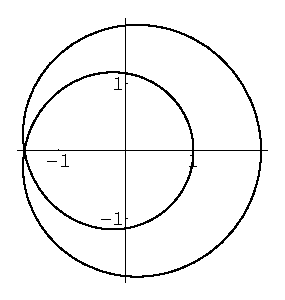
\includegraphics[width=0.3\textwidth]{fcv/integration/2sin2q4}
      \end{center}
      \caption{The contour.}
      \label{figure 2sin2q4}
    \end{figure}

    \begin{align*}
      \int_C z^{-1} \,\dd z
      &= \int_0^{4 \pi} \frac{1}{ r(\theta) \e^{\imath \theta } }  (r'(\theta) + \imath r(\theta)) \e^{\imath \theta} \,\dd \theta
      \\
      &= \int_0^{4 \pi} \left( \frac{ r'(\theta) }{ r(\theta) } + \imath \right)\,\dd \theta
      \\
      &= \left[ \log(r(\theta)) + \imath \theta \right]_0^{4 \pi}
    \end{align*}
    Since $r(\theta)$ does not vanish, the argument of $r(\theta)$ does not change in 
    traversing the contour and thus the logarithmic term has the same value at 
    the beginning and end of the path.
    \[
    \int_C z^{-1} \,\dd z = \imath 4 \pi
    \]
    This answer is twice what we found in part (a) because the contour goes 
    around the origin twice.
  \end{enumerate}
\end{Solution}




\begin{Solution}
  \label{solution bound z Log z z3+1}
  \begin{enumerate}
  \item 
    We parameterize the contour with $z = R \e^{\imath \theta}$ and bound the 
    modulus of the integral.
    \begin{align*}
      \left| \int_{C_R} \frac{ z + \Log z }{ z^3 + 1 } \,\dd z \right|
      &\leq \int_{C_R} \left| \frac{ z + \Log z }{ z^3 + 1 } \right|  
      \left| \dd z \right|
      \\
      &\leq \int_0^{2 \pi} \frac{ R + \ln R + \pi }{ R^3 - 1 }  R \,\dd \theta
      \\
      &= 2 \pi r \frac{ R + \ln R + \pi }{ R^3 - 1 }
    \end{align*}
    The upper bound on the modulus on the integral vanishes as $R \to \infty$.
    \[
    \lim_{R \to \infty}  2 \pi r \frac{ R + \ln R + \pi }{ R^3 - 1 } = 0
    \]
    We conclude that the integral vanishes as $R \to \infty$.
    \[
    \lim_{R \to \infty} \int_{C_R} \frac{ z + \Log z }{ z^3 + 1 } \,\dd z = 0
    \]
  \item 
    We parameterize the contour and bound the modulus of the integral.
    \[
    z = 2 \e^{\imath \theta}, \quad \theta \in [-\pi/2 \ldots \pi/2]
    \]
    \begin{align*}
      \left| \int_C \Log z \,\dd z \right|
      &\leq \int_C \left| \Log z \right| \left| \dd z \right|
      \\
      &= \int_{-\pi/2}^{\pi/2} |\ln 2 + \imath \theta| 2\,\dd \theta
      \\
      &\leq 2 \int_{-\pi/2}^{\pi/2} (\ln 2 + |\theta|)\,\dd \theta
      \\
      &= 4 \int_0^{\pi/2} (\ln 2 + \theta)\,\dd \theta
      \\
      &= \frac{\pi}{2} (\pi + 4 \ln 2)
    \end{align*}
  \item 
    We parameterize the contour and bound the modulus of the integral.
    \[
    z = R \e^{\imath \theta}, \quad \theta \in [\theta_0 \ldots \theta_0 + \pi]
    \]
    \begin{align*}
      \left| \int_C \frac{ z^2 - 1 }{ z^2 + 1 } \,\dd z \right| 
      &\leq \int_C \left| \frac{ z^2 - 1 }{ z^2 + 1 } \right|  \left| \dd z \right| 
      \\
      &\leq \int_{\theta_0}^{\theta_0 + \pi} \left| \frac{ R^2 \e^{\imath 2 \theta} - 1 }{ R^2 \e^{\imath 2 \theta} + 1 } \right| 
      \left| R\,\dd \theta \right| 
      \\
      &\leq R \int_{\theta_0}^{\theta_0 + \pi} \frac{ R^2 + 1 }{ R^2 - 1 }\,\dd \theta 
      \\
      &= \pi r \frac{R^2 + 1}{R^2 - 1}
    \end{align*}
  \end{enumerate}  
\end{Solution}







\begin{Solution}
  \label{solution parametric evaluation sqrt z}
  \begin{align*}
    \int_C f(z) \,\dd z
    &= \int_0^1 \sqrt{r}\,\dd r + \int_0^\pi \e^{\imath \theta/2}  \imath \e^{\imath \theta}\,\dd \theta + \int_1^0 \imath \sqrt{r}
    \,(-\dd r)
    \\
    &= \frac{2}{3} + \left( - \frac{2}{3} - \imath \frac{2}{3} \right)
    + \imath \frac{2}{3}
    \\
    &= 0
  \end{align*}
  The Cauchy-Goursat theorem does not apply because the function is not 
  analytic at $z = 0$, a point on the boundary.
\end{Solution}







\begin{Solution}
  \label{solution anti derivatives iz3 z-3}
  \begin{enumerate}
  \item 
    \begin{align*}
      \int_C \left( \imath z^3 + z^{-3} \right)\,\dd z
      &= \left[ \frac{\imath z^4}{4} - \frac{1}{2 z^2} \right]_{1+\imath}^\imath
      \\
      &= \frac{1}{2} + \imath
    \end{align*}
    In this example, the anti-derivative is single-valued.
  \item 
    \begin{align*}
      \int_C \sin^2 z \cos z \,\dd z
      &= \left[ \frac{\sin^3 z}{3} \right]_{\pi}^{\imath \pi}
      \\
      &= \frac{1}{3} \left( \sin^3(\imath \pi) - \sin^3(\pi) \right)
      \\
      &= - \imath \frac{\sinh^3(\pi)}{3}
    \end{align*}
    Again the anti-derivative is single-valued.
  \item 
    We choose the branch of $z^\imath$ with $-\pi/2 < \arg(z) < 3 \pi/2$.  This matches 
    the principal value of $z^\imath$ above the real axis and is defined 
    continuously on the path of integration.
    \begin{align*}
      \int_C z^\imath \,\dd z 
      &= \left[ \frac{z^{1 + \imath}}{1 + \imath} \right]_{\e^{\imath \pi}}^{\e^{\imath 0}}
      \\
      &= \left[ \frac{1 - \imath}{2} \e^{(1+\imath) \log z} \right]_{\e^{\imath \pi}}^{\e^{\imath 0}}
      \\
      &= \frac{1 - \imath}{2} \left( \e^{0}  - \e^{(1+\imath) \imath \pi} \right)
      \\
      &= \frac{1 + \e^{-\pi}}{2}  (1 - \imath)
    \end{align*}
  \end{enumerate}  
\end{Solution}







\raggedbottom
}
